% filepath: report/1-introduction.tex
\section{Introduction}
Halma is a strategy board game invented in the late 19th century, typically played on a checkered board by two players. The strategic depth of Halma, arising from its branching factor and long-term planning requirements, makes it an interesting testbed for artificial intelligence research. Figure~\ref{fig:halma} illustrates a typical Halma game setup in our code implementation.


\subsection{Rules}
In the original Halma rules, each player has multiple pawns and the objective is to transfer all of one's pieces from their starting corner or region to the diagonally opposite corner or region before the opponents do. Players take turns to move one pawn piece. Pieces can move to an adjacent square or jump over an adjacent piece (friendly or opponent) to the square immediately beyond it, with multiple jumps allowed in a single turn.
\begin{figure}[h]
    \centering
    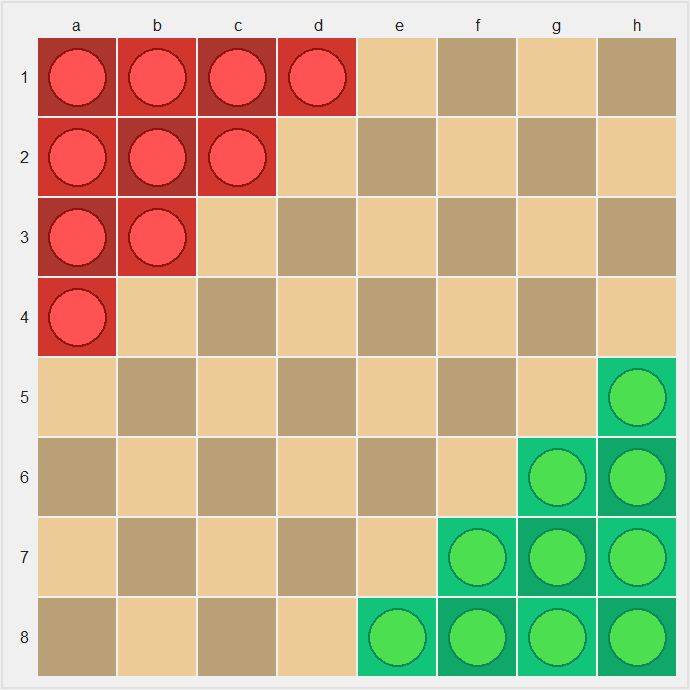
\includegraphics[width=1\columnwidth]{figures/halma.png}
    \caption{An example of a Halma game board and setup.}
    \label{fig:halma}
\end{figure}
\subsection{State Space}
In our game formulation, the board is 8$\times$8 and each player has 10 pawns. This means that the total number of state space is:
$$
\binom{64}{20} \times \binom{20}{10} = \frac{64!}{20! \cdot 44!} \times \frac{20!}{10! \cdot 10!} = \frac{64!}{44! \cdot 10! \cdot 10!} \approx 10^{28}
$$
\subsection{Motivation}

The motivation for this project is to use the knowledge about various agents in CS181 and deploy them in the scenario of Halma in practice. Also we seek to explore the impact of rules to our agents and see if there are any interesting findings when changing the rule a little bit. 

This report will introduce the design and implementation of several agents in CS181:
\begin{itemize}
    \item \textbf{Baseline agents:} \texttt{RandomPlayer} \item \textbf{Search agents:} \texttt{GreedyPlayer}
    \item \textbf{Adversary-Search agents:} \texttt{MinimaxPlayer} with alpha-beta pruning and optional local search heuristic.
    \item \textbf{Monte Carlo Tree Search:} \texttt{MCTSPlayer}\cite{DBLP:journals/corr/abs-2103-04931}
    \item \textbf{Reinforcement Learning agents:}
        \begin{itemize}
            \item \texttt{ApproximateQLearningPlayer}: Utilizes Q-learning with linear function approximation based on a rich set of handcrafted features and a tailored reward function.
            \item \texttt{Neural\_ApproximateQLearningPlayer}: Implements a Deep Q-Network (DQN)\cite{DBLP:journals/corr/MnihKSGAWR13} with a convolutional neural network\cite{DBLP:journals/corr/OSheaN15} for state representation, experience replay, and a target network.
        \end{itemize}
\end{itemize}

The competition results between these agents will be presented in this report. Moreover, we will discuss about how do we modify the rules and the corresponding interesting discoveries.
